% Options for packages loaded elsewhere
\PassOptionsToPackage{unicode}{hyperref}
\PassOptionsToPackage{hyphens}{url}
%
\documentclass[
]{article}
\usepackage{amsmath,amssymb}
\usepackage{iftex}
\ifPDFTeX
  \usepackage[T1]{fontenc}
  \usepackage[utf8]{inputenc}
  \usepackage{textcomp} % provide euro and other symbols
\else % if luatex or xetex
  \usepackage{unicode-math} % this also loads fontspec
  \defaultfontfeatures{Scale=MatchLowercase}
  \defaultfontfeatures[\rmfamily]{Ligatures=TeX,Scale=1}
\fi
\usepackage{lmodern}
\ifPDFTeX\else
  % xetex/luatex font selection
\fi
% Use upquote if available, for straight quotes in verbatim environments
\IfFileExists{upquote.sty}{\usepackage{upquote}}{}
\IfFileExists{microtype.sty}{% use microtype if available
  \usepackage[]{microtype}
  \UseMicrotypeSet[protrusion]{basicmath} % disable protrusion for tt fonts
}{}
\makeatletter
\@ifundefined{KOMAClassName}{% if non-KOMA class
  \IfFileExists{parskip.sty}{%
    \usepackage{parskip}
  }{% else
    \setlength{\parindent}{0pt}
    \setlength{\parskip}{6pt plus 2pt minus 1pt}}
}{% if KOMA class
  \KOMAoptions{parskip=half}}
\makeatother
\usepackage{xcolor}
\usepackage[margin=1in]{geometry}
\usepackage{color}
\usepackage{fancyvrb}
\newcommand{\VerbBar}{|}
\newcommand{\VERB}{\Verb[commandchars=\\\{\}]}
\DefineVerbatimEnvironment{Highlighting}{Verbatim}{commandchars=\\\{\}}
% Add ',fontsize=\small' for more characters per line
\usepackage{framed}
\definecolor{shadecolor}{RGB}{248,248,248}
\newenvironment{Shaded}{\begin{snugshade}}{\end{snugshade}}
\newcommand{\AlertTok}[1]{\textcolor[rgb]{0.94,0.16,0.16}{#1}}
\newcommand{\AnnotationTok}[1]{\textcolor[rgb]{0.56,0.35,0.01}{\textbf{\textit{#1}}}}
\newcommand{\AttributeTok}[1]{\textcolor[rgb]{0.13,0.29,0.53}{#1}}
\newcommand{\BaseNTok}[1]{\textcolor[rgb]{0.00,0.00,0.81}{#1}}
\newcommand{\BuiltInTok}[1]{#1}
\newcommand{\CharTok}[1]{\textcolor[rgb]{0.31,0.60,0.02}{#1}}
\newcommand{\CommentTok}[1]{\textcolor[rgb]{0.56,0.35,0.01}{\textit{#1}}}
\newcommand{\CommentVarTok}[1]{\textcolor[rgb]{0.56,0.35,0.01}{\textbf{\textit{#1}}}}
\newcommand{\ConstantTok}[1]{\textcolor[rgb]{0.56,0.35,0.01}{#1}}
\newcommand{\ControlFlowTok}[1]{\textcolor[rgb]{0.13,0.29,0.53}{\textbf{#1}}}
\newcommand{\DataTypeTok}[1]{\textcolor[rgb]{0.13,0.29,0.53}{#1}}
\newcommand{\DecValTok}[1]{\textcolor[rgb]{0.00,0.00,0.81}{#1}}
\newcommand{\DocumentationTok}[1]{\textcolor[rgb]{0.56,0.35,0.01}{\textbf{\textit{#1}}}}
\newcommand{\ErrorTok}[1]{\textcolor[rgb]{0.64,0.00,0.00}{\textbf{#1}}}
\newcommand{\ExtensionTok}[1]{#1}
\newcommand{\FloatTok}[1]{\textcolor[rgb]{0.00,0.00,0.81}{#1}}
\newcommand{\FunctionTok}[1]{\textcolor[rgb]{0.13,0.29,0.53}{\textbf{#1}}}
\newcommand{\ImportTok}[1]{#1}
\newcommand{\InformationTok}[1]{\textcolor[rgb]{0.56,0.35,0.01}{\textbf{\textit{#1}}}}
\newcommand{\KeywordTok}[1]{\textcolor[rgb]{0.13,0.29,0.53}{\textbf{#1}}}
\newcommand{\NormalTok}[1]{#1}
\newcommand{\OperatorTok}[1]{\textcolor[rgb]{0.81,0.36,0.00}{\textbf{#1}}}
\newcommand{\OtherTok}[1]{\textcolor[rgb]{0.56,0.35,0.01}{#1}}
\newcommand{\PreprocessorTok}[1]{\textcolor[rgb]{0.56,0.35,0.01}{\textit{#1}}}
\newcommand{\RegionMarkerTok}[1]{#1}
\newcommand{\SpecialCharTok}[1]{\textcolor[rgb]{0.81,0.36,0.00}{\textbf{#1}}}
\newcommand{\SpecialStringTok}[1]{\textcolor[rgb]{0.31,0.60,0.02}{#1}}
\newcommand{\StringTok}[1]{\textcolor[rgb]{0.31,0.60,0.02}{#1}}
\newcommand{\VariableTok}[1]{\textcolor[rgb]{0.00,0.00,0.00}{#1}}
\newcommand{\VerbatimStringTok}[1]{\textcolor[rgb]{0.31,0.60,0.02}{#1}}
\newcommand{\WarningTok}[1]{\textcolor[rgb]{0.56,0.35,0.01}{\textbf{\textit{#1}}}}
\usepackage{longtable,booktabs,array}
\usepackage{calc} % for calculating minipage widths
% Correct order of tables after \paragraph or \subparagraph
\usepackage{etoolbox}
\makeatletter
\patchcmd\longtable{\par}{\if@noskipsec\mbox{}\fi\par}{}{}
\makeatother
% Allow footnotes in longtable head/foot
\IfFileExists{footnotehyper.sty}{\usepackage{footnotehyper}}{\usepackage{footnote}}
\makesavenoteenv{longtable}
\usepackage{graphicx}
\makeatletter
\def\maxwidth{\ifdim\Gin@nat@width>\linewidth\linewidth\else\Gin@nat@width\fi}
\def\maxheight{\ifdim\Gin@nat@height>\textheight\textheight\else\Gin@nat@height\fi}
\makeatother
% Scale images if necessary, so that they will not overflow the page
% margins by default, and it is still possible to overwrite the defaults
% using explicit options in \includegraphics[width, height, ...]{}
\setkeys{Gin}{width=\maxwidth,height=\maxheight,keepaspectratio}
% Set default figure placement to htbp
\makeatletter
\def\fps@figure{htbp}
\makeatother
\setlength{\emergencystretch}{3em} % prevent overfull lines
\providecommand{\tightlist}{%
  \setlength{\itemsep}{0pt}\setlength{\parskip}{0pt}}
\setcounter{secnumdepth}{-\maxdimen} % remove section numbering
\ifLuaTeX
  \usepackage{selnolig}  % disable illegal ligatures
\fi
\usepackage{bookmark}
\IfFileExists{xurl.sty}{\usepackage{xurl}}{} % add URL line breaks if available
\urlstyle{same}
\hypersetup{
  pdftitle={R Markdown},
  pdfauthor={Charles},
  hidelinks,
  pdfcreator={LaTeX via pandoc}}

\title{R Markdown}
\author{Charles}
\date{2025-04-02}

\begin{document}
\maketitle

{
\setcounter{tocdepth}{2}
\tableofcontents
}
\section{\texorpdfstring{\textbf{Chapter
Two}}{Chapter Two}}\label{chapter-two}

\section{Header 1 (Main heading)}\label{header-1-main-heading}

\subsection{Header 2 (Sub heading)}\label{header-2-sub-heading}

\subsubsection{Header 3 (Sub heading)}\label{header-3-sub-heading}

\subsection{Creating a list}\label{creating-a-list}

\subsubsection{Unordered list}\label{unordered-list}

\begin{itemize}
\tightlist
\item
  This is the first line

  \begin{itemize}
  \tightlist
  \item
    This is a sub-line
  \item
    This is another sub-line
  \end{itemize}
\item
  This actually goes to the outer level
\item
  This is definitely at the outer level
\end{itemize}

\subsubsection{Ordered list}\label{ordered-list}

\begin{itemize}
\tightlist
\item
  First line
\item
  Second line

  \begin{itemize}
  \tightlist
  \item
    nested line
  \end{itemize}
\end{itemize}

\begin{enumerate}
\def\labelenumi{\arabic{enumi}.}
\tightlist
\item
  Charles is a good man and ambitious about his dreams.
\item
  numbered
\item
  list
\end{enumerate}

\subsection{Creating Tables}\label{creating-tables}

\begin{longtable}[]{@{}lcr@{}}
\toprule\noalign{}
Name & Gender & Occupation \\
\midrule\noalign{}
\endhead
\bottomrule\noalign{}
\endlastfoot
Charles Kwame Appiah & Male & Renewable Energy Engineer \\
Richmond Amoah & \emph{Male} & \emph{Fashion} \\
Ann Amoah & \emph{Female} & \emph{Doctor} \\
\end{longtable}

\subsubsection{Italics}\label{italics}

\emph{Charles is good at what he does}

\subsubsection{Bold}\label{bold}

\textbf{Charles is always finding new ways to learn new things everyday}

\subsubsection{Creating a link}\label{creating-a-link}

\href{https://github.com/ckappiah1999/Charles_Nana}{Ckappiah1999}

\subsection{Inseritng a picture}\label{inseritng-a-picture}

We insert images like this, starting with the exclamation mark !, adding
a square bracket {[}{]} to contain the text of the image and adding the
path to the image.

\begin{figure}
\centering
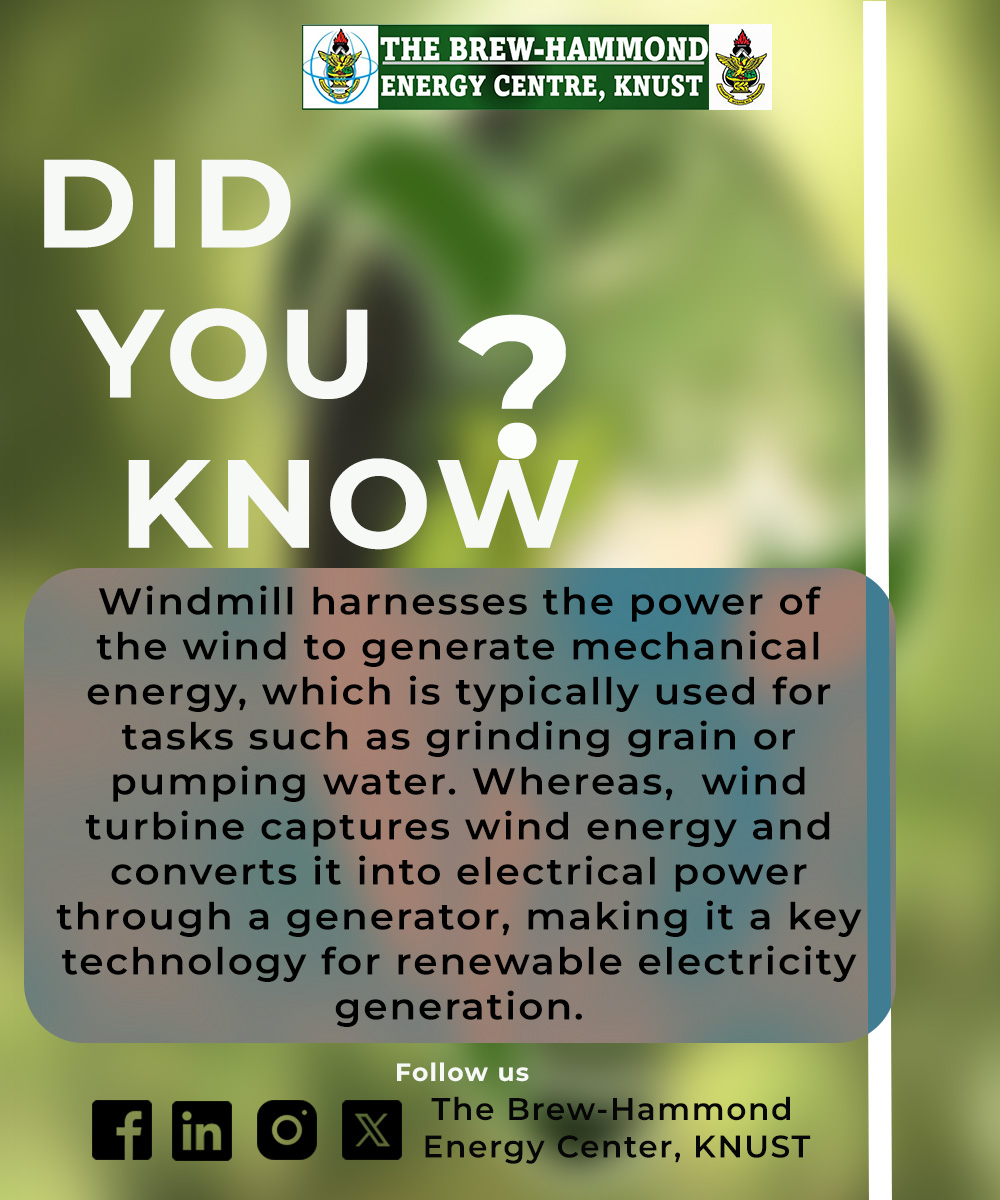
\includegraphics[width=0.3\textwidth,height=\textheight]{Wind.jpg}
\caption{Did you know}
\end{figure}

\subsection{Inline code}\label{inline-code}

\texttt{Click\ on\ this\ link\ to\ get\ access\ to\ my\ account\ on}
\href{https://github.com/ckappiah1999/Charles_Nana}{Github}

This is some text {[}with a link{]}{[}interesting{]}.

\begin{quote}
This is a block quote
\end{quote}

\subsubsection{Creating a chunk}\label{creating-a-chunk}

\begin{Shaded}
\begin{Highlighting}[]
\FunctionTok{data}\NormalTok{(presidents)}
\FunctionTok{str}\NormalTok{(}\FunctionTok{as.data.frame}\NormalTok{(presidents))}
\end{Highlighting}
\end{Shaded}

\begin{verbatim}
## 'data.frame':    120 obs. of  1 variable:
##  $ x: Time-Series  from 1945 to 1975: NA 87 82 75 63 50 43 32 35 60 ...
\end{verbatim}

\begin{Shaded}
\begin{Highlighting}[]
\NormalTok{pre }\OtherTok{\textless{}{-}}\NormalTok{ presidents}

\FunctionTok{print}\NormalTok{(pre)}
\end{Highlighting}
\end{Shaded}

\begin{verbatim}
##      Qtr1 Qtr2 Qtr3 Qtr4
## 1945   NA   87   82   75
## 1946   63   50   43   32
## 1947   35   60   54   55
## 1948   36   39   NA   NA
## 1949   69   57   57   51
## 1950   45   37   46   39
## 1951   36   24   32   23
## 1952   25   32   NA   32
## 1953   59   74   75   60
## 1954   71   61   71   57
## 1955   71   68   79   73
## 1956   76   71   67   75
## 1957   79   62   63   57
## 1958   60   49   48   52
## 1959   57   62   61   66
## 1960   71   62   61   57
## 1961   72   83   71   78
## 1962   79   71   62   74
## 1963   76   64   62   57
## 1964   80   73   69   69
## 1965   71   64   69   62
## 1966   63   46   56   44
## 1967   44   52   38   46
## 1968   36   49   35   44
## 1969   59   65   65   56
## 1970   66   53   61   52
## 1971   51   48   54   49
## 1972   49   61   NA   NA
## 1973   68   44   40   27
## 1974   28   25   24   24
\end{verbatim}

\begin{Shaded}
\begin{Highlighting}[]
\NormalTok{f }\OtherTok{\textless{}{-}} \ControlFlowTok{function}\NormalTok{(x) }\FunctionTok{ifelse}\NormalTok{(x }\SpecialCharTok{\%\%} \DecValTok{2} \SpecialCharTok{==} \DecValTok{0}\NormalTok{, x}\SpecialCharTok{**}\DecValTok{2}\NormalTok{, x}\SpecialCharTok{**}\DecValTok{3}\NormalTok{)}
\FunctionTok{f}\NormalTok{(}\DecValTok{2}\SpecialCharTok{:}\DecValTok{20}\NormalTok{)}
\end{Highlighting}
\end{Shaded}

\begin{verbatim}
##  [1]    4   27   16  125   36  343   64  729  100 1331  144 2197  196 3375  256
## [16] 4913  324 6859  400
\end{verbatim}

\subsubsection{creating section}\label{creating-section}

{[}this section{]}{[}@ckappiah1999.com{]}

\subsubsection{Creating biography}\label{creating-biography}

bibliography: bibliography.bib \ldots{} ---

{[}@ckappiah1999, chapter 4{]}

bibliography: bibliography.bib csl: biomed-central.csl \ldots{} ---

{[}@ckappiah1999.com{]}

Charles

\subsubsection{Adding citation}\label{adding-citation}

We can add citation like this \footnote{Done for the day}

\begin{Shaded}
\begin{Highlighting}[]
\FunctionTok{data}\NormalTok{(cars)}
\FunctionTok{summary}\NormalTok{(cars)}
\end{Highlighting}
\end{Shaded}

\begin{verbatim}
##      speed           dist       
##  Min.   : 4.0   Min.   :  2.00  
##  1st Qu.:12.0   1st Qu.: 26.00  
##  Median :15.0   Median : 36.00  
##  Mean   :15.4   Mean   : 42.98  
##  3rd Qu.:19.0   3rd Qu.: 56.00  
##  Max.   :25.0   Max.   :120.00
\end{verbatim}

\begin{Shaded}
\begin{Highlighting}[]
\FunctionTok{sum}\NormalTok{(cars)}
\end{Highlighting}
\end{Shaded}

\begin{verbatim}
## [1] 2919
\end{verbatim}

\begin{Shaded}
\begin{Highlighting}[]
\FunctionTok{str}\NormalTok{(cars)}
\end{Highlighting}
\end{Shaded}

\begin{verbatim}
## 'data.frame':    50 obs. of  2 variables:
##  $ speed: num  4 4 7 7 8 9 10 10 10 11 ...
##  $ dist : num  2 10 4 22 16 10 18 26 34 17 ...
\end{verbatim}

The mean of the distant in the cars dataset is 42.98

\subsubsection{Calling the knit package}\label{calling-the-knit-package}

\begin{Shaded}
\begin{Highlighting}[]
\FunctionTok{library}\NormalTok{(knitr)}
\FunctionTok{kable}\NormalTok{(}\FunctionTok{head}\NormalTok{(cars))}
\end{Highlighting}
\end{Shaded}

\begin{longtable}[]{@{}rr@{}}
\toprule\noalign{}
speed & dist \\
\midrule\noalign{}
\endhead
\bottomrule\noalign{}
\endlastfoot
4 & 2 \\
4 & 10 \\
7 & 4 \\
7 & 22 \\
8 & 16 \\
9 & 10 \\
\end{longtable}

\begin{Shaded}
\begin{Highlighting}[]
\FunctionTok{set.seed}\NormalTok{(}\DecValTok{123}\NormalTok{)  }\CommentTok{\# Ensures reproducibility initially}
\NormalTok{random\_numbers }\OtherTok{\textless{}{-}} \FunctionTok{rnorm}\NormalTok{(}\DecValTok{200}\NormalTok{)  }\CommentTok{\# Generate 100 random values}
\FunctionTok{head}\NormalTok{(random\_numbers)  }\CommentTok{\# Display first few numbers}
\end{Highlighting}
\end{Shaded}

\begin{verbatim}
## [1] -0.56047565 -0.23017749  1.55870831  0.07050839  0.12928774  1.71506499
\end{verbatim}

\begin{Shaded}
\begin{Highlighting}[]
\NormalTok{mean\_random }\OtherTok{\textless{}{-}} \FunctionTok{mean}\NormalTok{(random\_numbers)}
\NormalTok{mean\_random  }\CommentTok{\# Compute and display the mean}
\end{Highlighting}
\end{Shaded}

\begin{verbatim}
## [1] -0.008570445
\end{verbatim}

\end{document}
